
\subsection{Example}
\begin{align*}
    F(z) = \frac{1}{(z+1)(z+2)^2}
\end{align*}
Want to find $f: \mathbb{R}_+ \rightarrow \mathbb{C}$ auch that $\mathcal{L}[f] = F$
Two ways to do this:
\begin{enumerate}
    \item Partial fonction decomposition
    \begin{align*}
        \frac{1}{(z+1)(z+2)^2} = \frac{1}{z+1} - \frac{1}{z+2} - \frac{1}{(z+2)^2} \\ = e^{-t} - e^{-2t} - te^{-2t}
    \end{align*}
    Here is a few example how to do : \\
    \begin{center}
        
    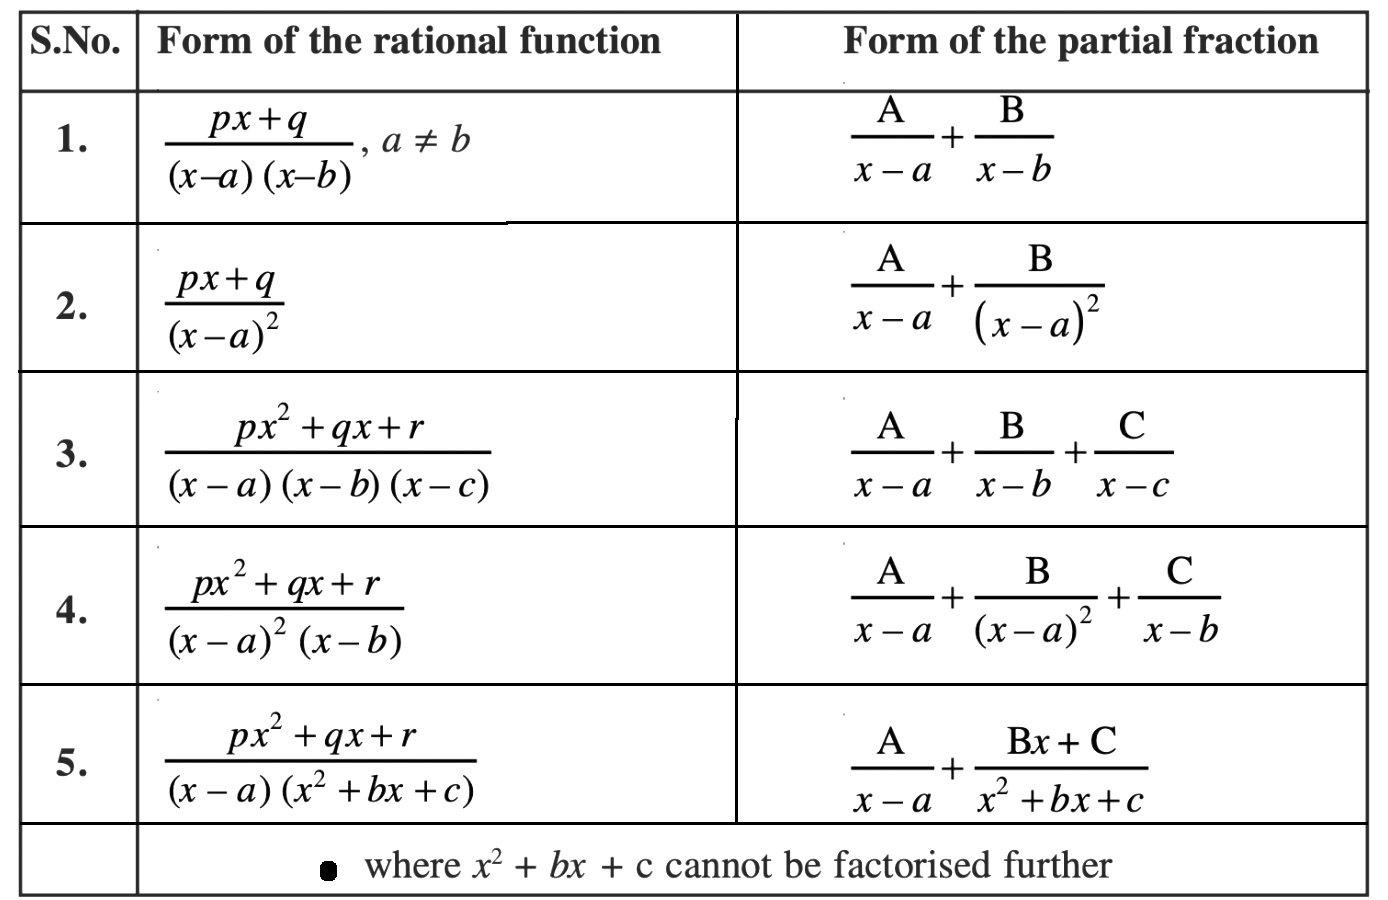
\includegraphics[width=250px]{integration-by-partial-fractions.png}
    \end{center}
    \item Inverse laplace transdorm and residue theorem 
    \begin{align*}
        f(t) = \frac{1}{2 \pi}\int_{-\infty}^\infty F(\gamma + is) e^{(\gamma + is)t}ds
    \end{align*}
    let $h(z) = F(z)e^{zt}$. Poles for $h$ are $z = -1$ and $z = -2$
    Now we choose $\gamma =0. $
    \begin{itemize}
        \item $F$ is holomorphic on $\{Re > -1\}$
        \item $\int_{-\infty}^\infty|F(\gamma + is)|ds < \infty$
    \end{itemize}
    Inverse Laplace transform 
    \begin{align*}
        f(t) = \frac{1}{2 \pi}\int_{-\infty}^\infty h(\gamma + is)ds
    \end{align*}
\end{enumerate}

\subsection{Applications to partial differential equations (PDES)}
As for ODES we will apply the theory of Laplace and Fourier transform to solve initial-boundary value problems for \textbf{linear} PDES while \textbf{constant coefficients},eg. licat equation
\begin{align*}
    \frac{\partial u}{\partial t}(x,t) - \frac{\partial^2u}{\partial x^2}u(x,t) = f(x,t) \ \ \text{for } t > 0 \text{ and } x \in (0,L) \\
    u(x,0) = u_0(x) \text{ (initial condition)} \\
    u(0,t) =0, u(L,t) = 0 \text{ (boundary condition)}
\end{align*}
Describe the evolution of temperature $u$ of a one-dimensional rod of length $L$ with heat source $f$ and fixed temperature at the endpoints $0,L$

\text{General procedure} that we will follows
\begin{itemize}
    \item  \textbf{Fourier series} if space or time domain bounded 
    \item \textbf{Fourier transform} if space or time domain $\mathbb{R}$
    \item \textbf{Laplace transform} if space or time domain $\mathbb{R}_+$
\end{itemize}

\subsubsection{Fourier series recapitulation}
We want to decompose $f: [0, 1] \rightarrow \mathbb{R}$ as an infinite sum of ascillativy functions. Basics functions
\begin{itemize}
    \item \begin{align*}
        \sin(\frac{2 \pi u}{L}x) \ \text{ where } u \geq 1
    \end{align*}
    \item \begin{align*}
        \cos(\frac{2 \pi u}{L}x) \ \text{ where } u \geq 0
    \end{align*}
\end{itemize}
\textbf{Orthogonality} Inner product : \begin{align*}
    <f,y> := \int_0^L f(x)g(x)dx
\end{align*}
\begin{itemize}
    \item \begin{align*}
        <\sin(\frac{2 \pi u}{L}x), \sin(\frac{2 \pi w}{L}x)> = \begin{cases}
            L/ 2 \ \text{ if w=u}
            \\ 0 \ \text{ otherwise}
        \end{cases}
    \end{align*}
    \item \begin{align*}
        \text{some for } <\cos(\frac{2 \pi u}{L}x), \cos(\frac{2 \pi w}{L}x)>
    \end{align*}
    \item \begin{align*}
        <\sin(\frac{2 \pi u}{L}x), \cos(\frac{2 \pi w}{L}x)> = 0 \ \text{for all } u,w
    \end{align*}
\end{itemize}
We will use these fcts as orthogonal basis to decompose other functions via trigonometric (Fourier) series
Given $f: [0,L] \rightarrow \mathbb{R}$ piecewise continuous, can be write  
\begin{align*}
    f(x) = \frac{a_0}{2} + \sum_{u=1}^\infty [a_u \cos(\frac{2 \pi u}{L}x) + b_u \sin(\frac{2 \pi u}{L}x)]
\end{align*}
The answer is yes

To "guess" the form of the coefficients $a_u$ and $b_u$, we assume $f$ already has this form. Then we can (formally) compute the following using orthogonality. 
\begin{itemize}
    \item \begin{align*}
        \int_0^L f(x) dx = \frac{L}{2}a_0
    \end{align*}
    \item \begin{align*}
        \int_0^L f(x) \cos(\frac{2 \pi u}{L}x)dx = \frac{L}{2}a_u \ \text{ where } u \geq 1
    \end{align*}
    \item \begin{align*}
        \int_0^L f(x) \sin(\frac{2 \pi u}{L}x)dx = \frac{L}{2}b_u \ \text{ where } u \geq 1
    \end{align*}
\end{itemize}
This suppests to define 
\begin{align*}
    a_u = \frac{2}{L} \int_0^L f(x) \cos(\frac{2 \pi u}{L}x)dx \ \text{ where } u \geq 0 \\
    b_u = \frac{2}{L} \int_0^L f(x) \sin(\frac{2 \pi u}{L}x)dx \ \text{ where } u \geq 1
\end{align*}
Trigonomertic Fouries decomposition. Define $f_N: [0,L] \rightarrow \mathbb{R}$
\begin{align*}
    f_N(x) = \frac{a_0}{2} + \sum_{u=1}^N [a_u \cos(\frac{2 \pi u}{L}x) + b_u \sin(\frac{2 \pi u}{L}x)dx]
\end{align*}
where $a_u$ and $b_u$ are as above, ehre $f: [0,L] \rightarrow \mathbb{R}$ is piecewise continuous. Then 
\begin{itemize}
    \item $f_N(x) \rightarrow f(x)$ as $N \rightarrow \infty$ at every $x \in [0,L]$ where $f$ is differentiable
    \item $f_N(x) \rightarrow \frac{f(x+) + f(x-)}{2}$ when $x$ is a jump discoutinuity of $f$
    \item \begin{align*} \lim_{u\rightarrow \infty} \int_0^L|f_N(x)-f(x)|dx = 0 \end{align*}
\end{itemize}

\subsubsection{special cases }
\begin{itemize}
    \item Assume $f$ odd $(f(-x) = -f(x)$ for all $x \in [0,L])$ Then $a_u = 0$ for every $u \geq 0$ and 
    \begin{align*}
        f(x) = \sum_{u=1}^\infty b_u \sin(\frac{2 \pi u}{L}x)
    \end{align*} where 
    \begin{align*}
        b_u = \frac{4}{L}\int_0^{\frac{L}{2}} f(x)\sin(\frac{2\pi u}{L}x)dx
    \end{align*}
    \item Assume $f$ even. then $b_u=0$ for all $u \geq 1$ and 
    \begin{align*}
        f(x) = \frac{a_0}{2} + \sum_{u=1}^\infty a_u \cos(\frac{2 \pi u}{L}x)
    \end{align*} where 
    \begin{align*}
        a_u = \frac{4}{L}\int_0^{\frac{L}{2}} f(x) \cos(\frac{2 \pi u}{L}x) dx
    \end{align*}
\end{itemize}